\section{CIVIS Platform  Development} 
 
The development (implementation) of the CIVIS platform was started in May 2015 \citep{Huang2015c} and continued in the third year's WP3 activities. At the time of writing this deliverable (Jun 2016), the development is completed with some minor updates took place in the past month.
% 
The JavaScript (JS) programming language\footnote{\url{http://www.crockford.com/javascript/javascript.html}} is used for development at both front- and back-ends. 
The platforms and technologies mentioned in this section are all free and open source. 

\subsection{CIVIS Front-End as a Hybrid Application} 

The CIVIS front-end (YouPower) is developed as a hybrid (cross-platform) mobile application using Ionic\footnote{\url{http://ionicframework.com/}}, an HTML5 front-end development framework built with SASS\footnote{\url{http://sass-lang.com/}} and optimized for AngularJS\footnote{\url{https://angularjs.org/}} (a.k.a Angular). 
% 
The Ionic framework comes with native-styled mobile UI elements and layouts, and handles the look and feel and the UI interactions the app needs in order to be compelling\footnote{\url{http://ionicframework.com/docs/guide/}}. 

The energy data visualizations are built using the HighCharts library\footnote{\url{http://www.highcharts.com/}}, wrapped using the {\tt highchart-ng} directives for Ionic\footnote{\url{https://github.com/pablojim/highcharts-ng}}.

Angular as a JavaScript framework provides directives (extensions of HTML attributes) and two-way data binding (binds input or output data of the view to a model) that simplify the app development with MVC architecture. The ``Current Actions'' in the ``Action List'', for example, are rendered with the following HTML code: 

% 
{\scriptsize  
\begin{verbatim}
<div class="...">Current Actions ({{_.size(currentUser.actions.inProgress)}})</div>
<a class="..." ng-repeat="action in currentUser.actions.inProgress" ng-href="#/app/actions/active/{{$index}}">
   {{getActionPoints(action)}} {{action.name}}
</a>
\end{verbatim}
}
% 
\noindent where {\footnotesize  \verb currentUser.actions.inProgress } is a model of a list ({\footnotesize  \verb array }) of the user's actions (the data) that are dynamically loaded into the corresponding controller from the CIVIS back-end at runtime. 
The Angular directive  {\footnotesize  \verb ng-repeat } then iterates through the list, takes each element as an  {\footnotesize  \verb action }, and displays the data in the view. The function {\footnotesize \verb getActionPoints(action) } is defined in the controller. It is a good example of two-way data binding where the value of {\footnotesize  \verb action } (the model) is passed on from the view to the controller, and the function returns the result form the controller to the view. 

\subsection{CIVIS Back-End}

An early version of YouPower\footnote{Branch study-protoype \url{https://github.com/CIVIS-project/YouPower/tree/study-prototype}, 
\url{https://app.civisproject.eu/frontend.html}} has its back-end on Firebase\footnote{\url{https://youpower.firebaseio.com/}} to have a quick set-up.  
For the same reason, the YouPower back-end development is first deployed on Heroku\footnote{\url{https://www.heroku.com/}}. In July 2015, TU Delft finished preparing a virtual machine for CIVIS, so the WP3 back-end is currently hosted by a TU Delft server at {\footnotesize\url{http://civis.tbm.tudelft.nl}}. The CIVIS app back-end interacts with the IT platform developed in WP4, from which it fetches relevant data to be used in the front-end. This is particularly relevant for visualization of energy consumption/production data, energy price data and donation programme data. The availability of such data through the WP4 platform represents therefore a pre-condition for the ability of the app to correctly visualize such information.

The YouPower back-end is developed using the Node.js\footnote{\url{https://nodejs.org/}} platform, a well-known JS based open source runtime environment for server-side applications. 
The platform is easily extensible and has a repository of libraries that support fast web development.
MongoDB\footnote{\url{https://mongodb.org/}} is used as the back-end database. It is document-oriented, and has flexible data schema and expressive query language. 
A list of the data models at the back-end can be found at {\footnotesize\url{https://github.com/CIVIS-project/YouPower/tree/master/backend/models}}. 
Figure~\ref{fig:datamodel} shows the data model schema.
%
\begin{figure}
\centering
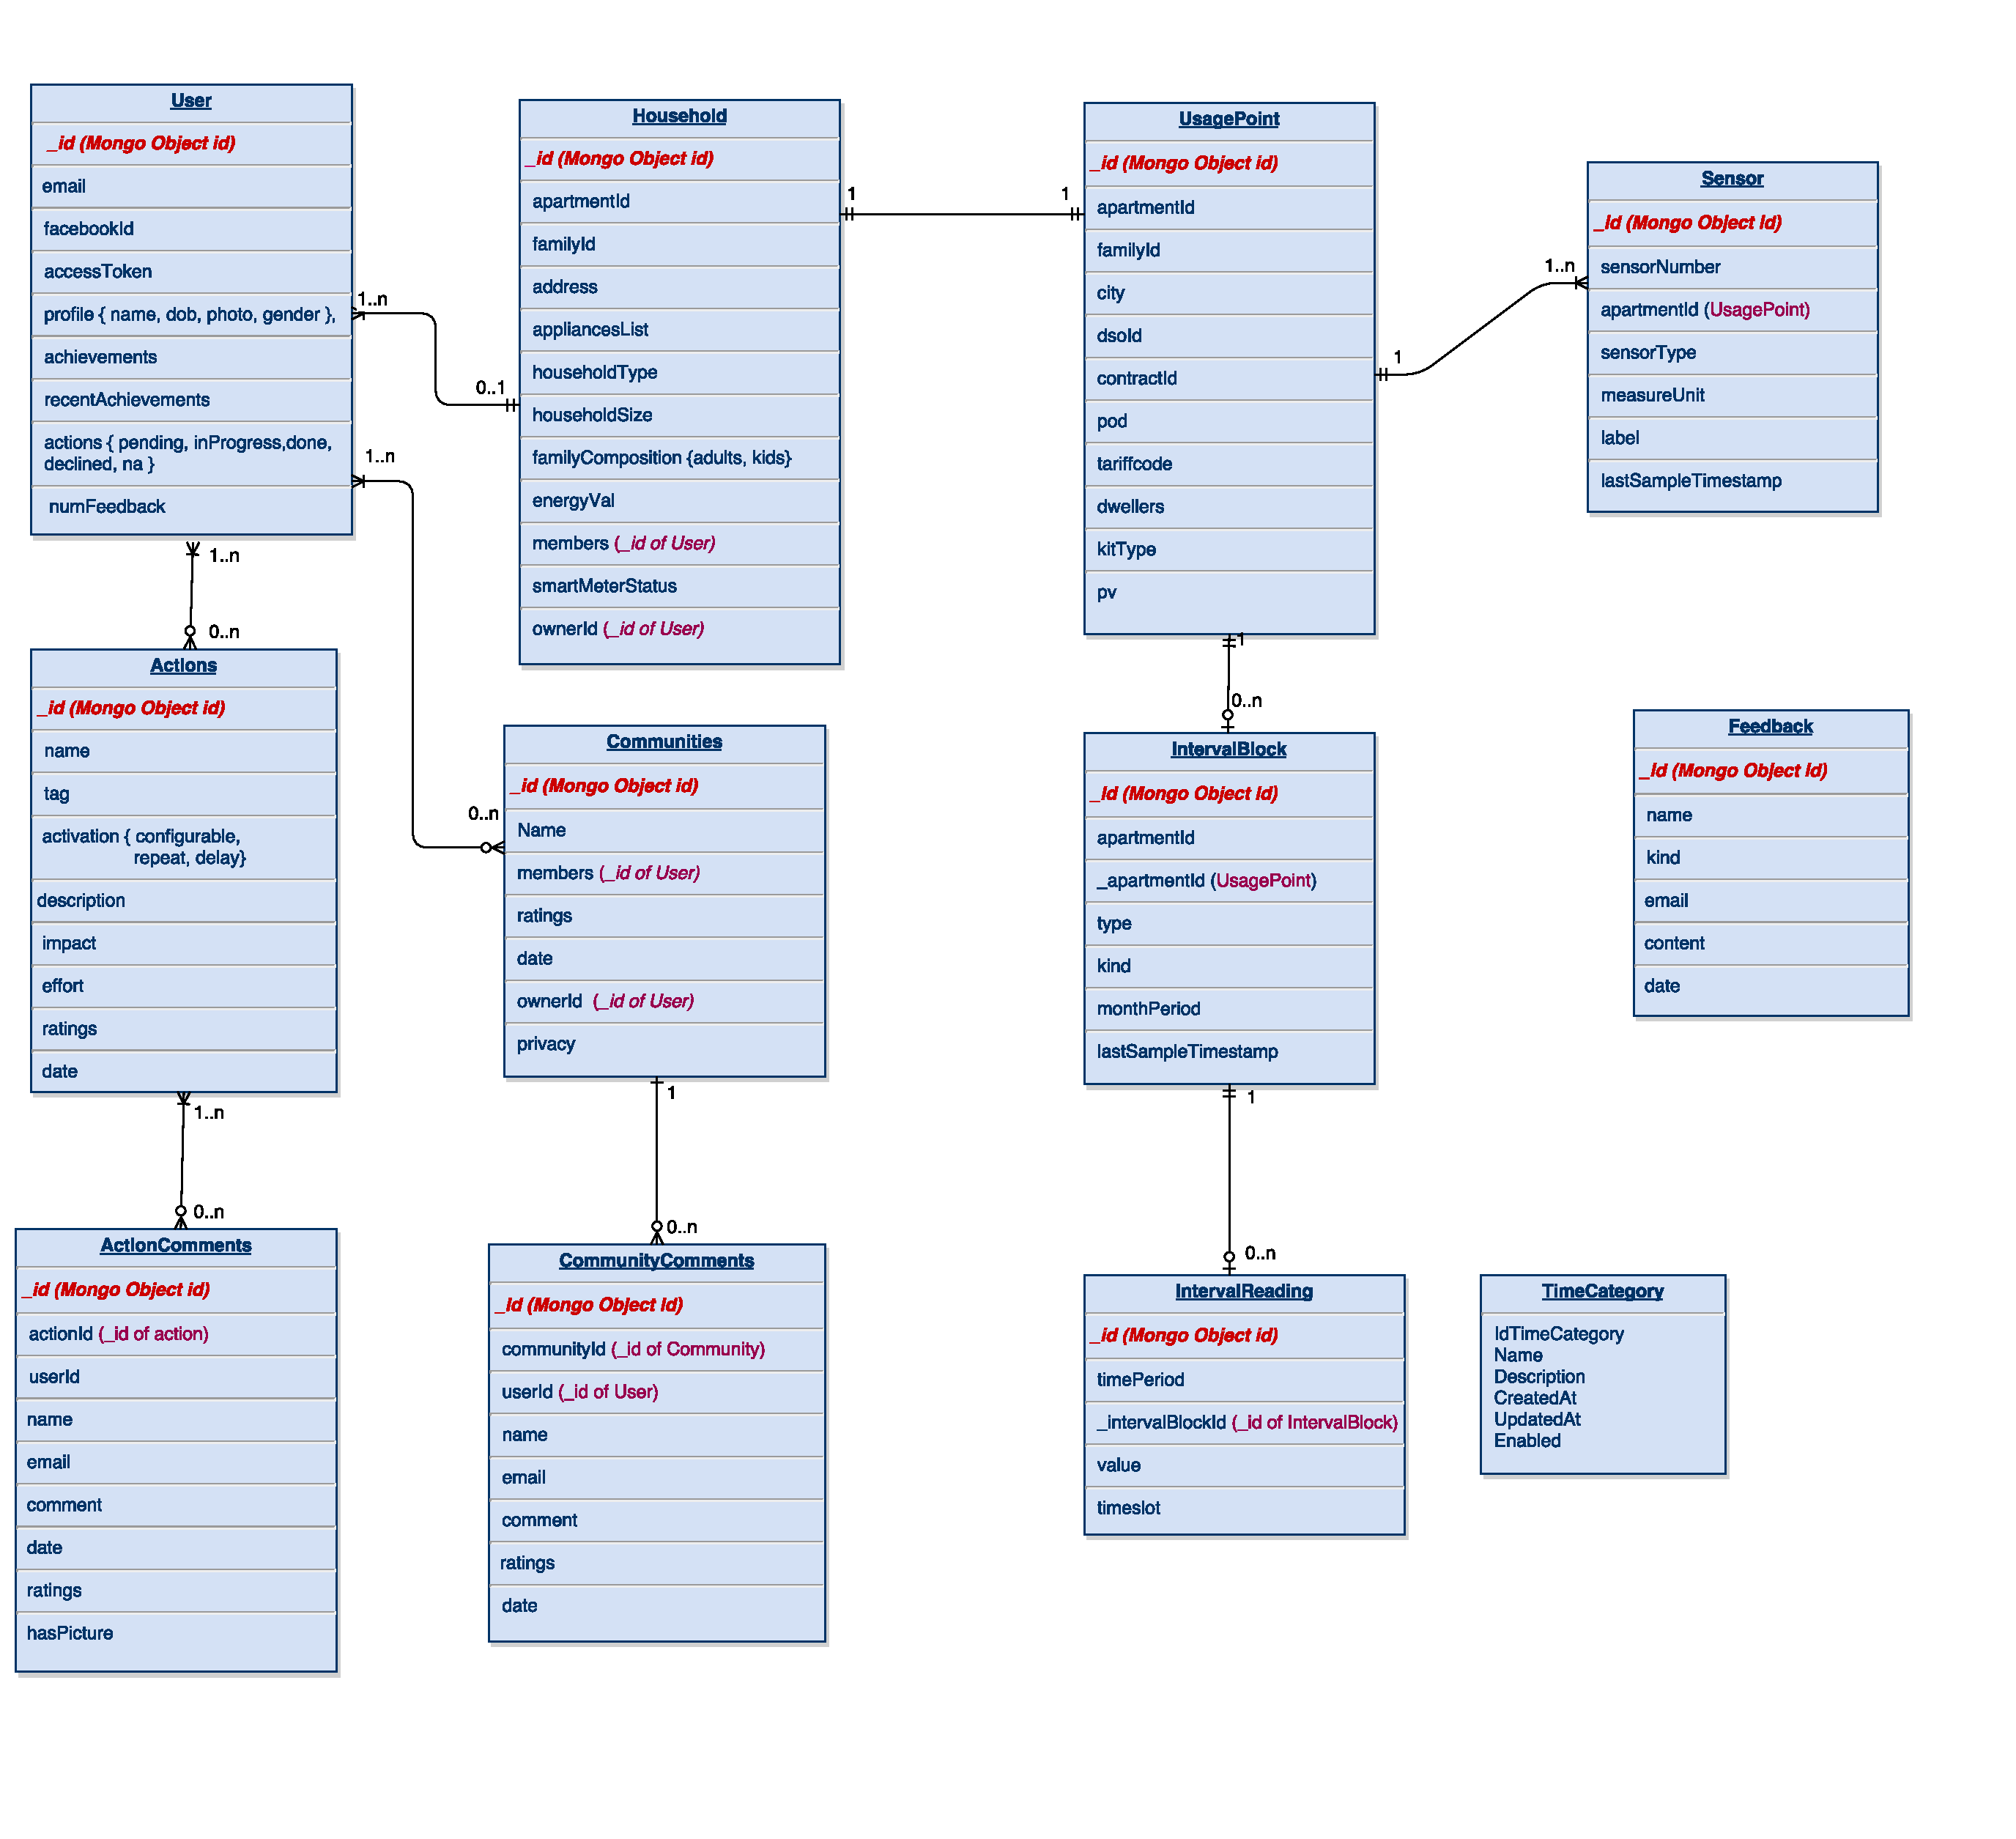
\includegraphics[height=\linewidth,angle=90]{img/datamodel_larger}
\caption{YouPower back-end data model schema}
\label{fig:datamodel}
\end{figure} 
% 
The noteworthy Node.js libraries we use for the back-end development are as follows:
\begin{itemize}
\item Async.js\footnote{\url{https://github.com/caolan/async}}, which makes managing and combining asynchronous tasks easier. 
\item Express.js\footnote{\url{http://expressjs.com/}}, a Node.js application server framework we use as a basis for the REST API. 
\item Mocha\footnote{\url{https://mochajs.org/}}, a JavaScript unit test framework. 
\item Mongoose\footnote{\url{http://mongoosejs.com/}}, a MongoDB driver for Node.js. It provides a schema-based solution to model data. 
\item Passport.js\footnote{\url{http://passportjs.org/}}, for handling authentication of REST API requests for Node.js, both local (username password) and Facebook. 
%\item Underscore.js, handy library that extends JavaScript with useful functions. 
\item Ionic Push\footnote{\url{https://apps.ionic.io/landing/push}}, for sending dynamic push notifications. 
\item APIDOC script\footnote{\url{http://apidocjs.com/}}, for inline documentation for the REST API. 
\end{itemize}

The YouPower back-end REST API documentation can be found at {\footnotesize\url{http://civis.tbm.tudelft.nl/apidoc/}}. 
% 


\begin{figure}
\centering
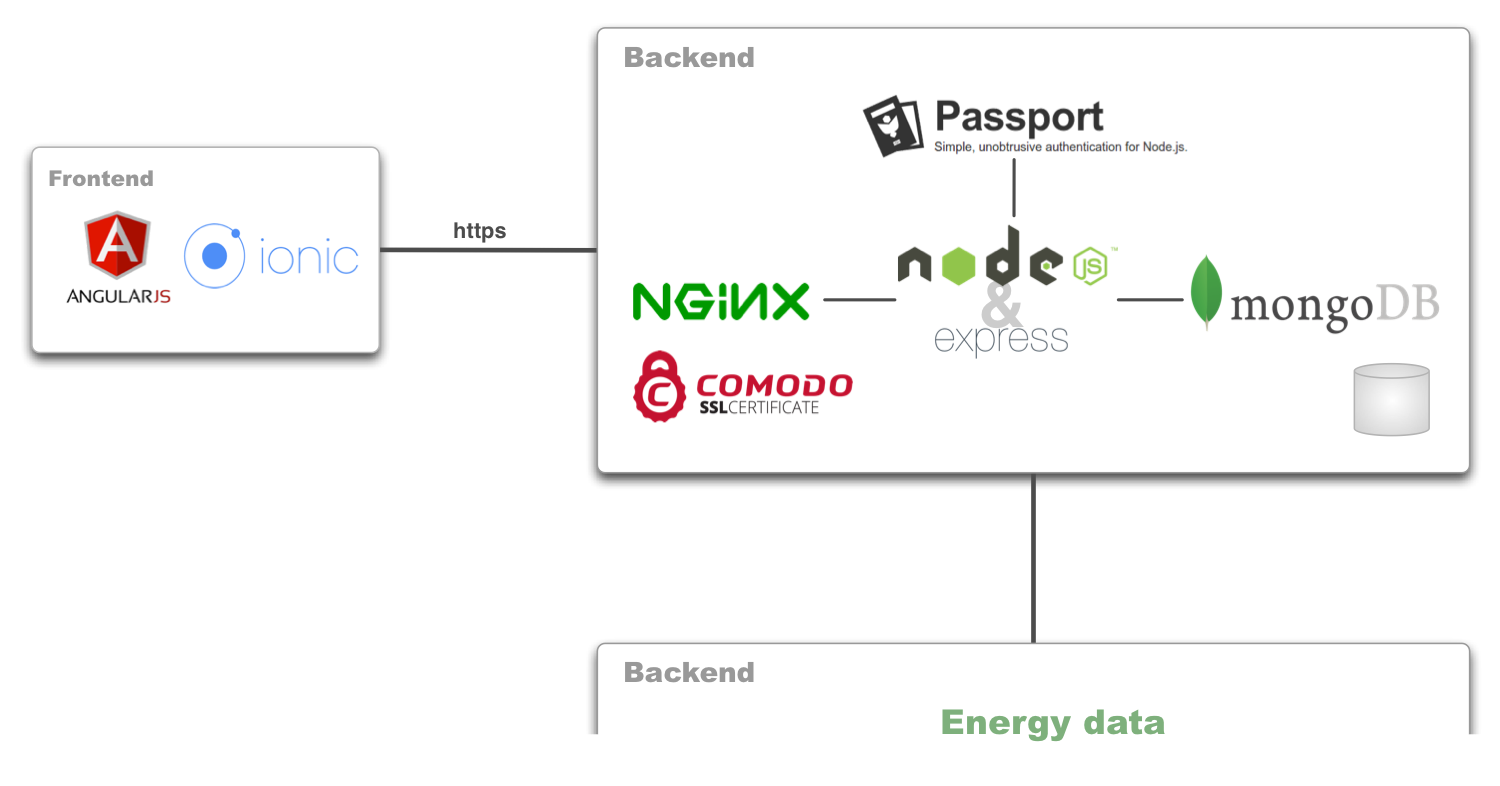
\includegraphics[width=0.9\linewidth]{img/tech}
\caption{WP3}
\label{fig:ScreenShot2015-11-09at18}
\end{figure}


\subsection{Resources}